\chapter{Integration of an ICPC Detector}\label{chap:integration}

The n-type segmented point-contact germanium detector served as an effective test bench for the Compton Scanner. Building on this success, the Compton Scanner was integrated with a LEGEND ORTEC\textsuperscript{\tiny\textregistered} p-type inverted coaxial point contact detector -- \IC{}. 

The detector was mounted in an ORTEC\textsuperscript{\tiny\textregistered} PopTop\textsuperscript{\tiny TM} cryostat with an attached cooling rod. This integrated system housed the detector in vacuum, along with an easily-accessible charge sensitive preamplifier and high-voltage (HV) filter. A single cable bundle exited the PopTop via a feedthrough which included coaxial cables for signal readout and pulser input, a SHV connector for HV input and a DB-9 connector for the low-voltage (LV) input to the preamplifier. The signal cable is connected to an analog-to-digital converter (ADC) (Section~\ref{sec:ic_det_intru}). To reach the cryogenic temperatures necessary for detector operation, the attached cooling rod was immersed in a 30L liquid nitrogen (LN$_2$) main dewar. In this system LN$_2$ boiled off at a rate of approximately 5\,L/day. Thus, a 150\,L LN$_2$ dewar was attached to refill the main dewar every three days. Four PT-100 thermoresistors~\cite{pt100} were placed along the length of the cooling rod and were connected to a temperature monitor (LAKE SHORE\textsuperscript{\tiny\textregistered} Model 218~\cite{lakeshore}) which was readout by the NetCom serial server of the motor control system. These data were used to determine the LN$_2$ level of the main dewar.  Each of these systems, ADC, LN$_2$ dewars, temperature monitor, and HV and LV supplies were placed in the periphery of the detector as shown in Fig.~\ref{fig:full_setup}. A table was built around the main dewar, with a hole cut out for the cryostat. The rotational motor and Compton Scanner frame were mounted on this table and the centers of the frame and the detector were aligned (See Section~\ref{sec:centeralignment}).

A PC was connected to the ADC with fiber optics to eliminate any noise-coupling into the system. The PC ran all data acquisition (DAQ) scripts and stored data locally on a 1.3\,TB solid state drive. Monitoring scripts on the DAQ PC collected and stored HV, temperature sensor, hard drive and Compton Scanner motor position data at 60\,s intervals. A compilation of the relevant data was live-streamed and available online from any web browser (Section~\ref{sec:monitoring}). All systems, except the ADC and the Compton Scanner camera system (due to noise coupling, Section~\ref{sec:noise}) were powered by a XANTO 3000R universal power supply (UPS)~\cite{ups} and had common ground. The cameras were connected to the same Ethernet switch as the DAQ PC and NetCom serial server and one sync line from each camera was connected to the ADC.

\begin{figure}[htb]
    \centering
    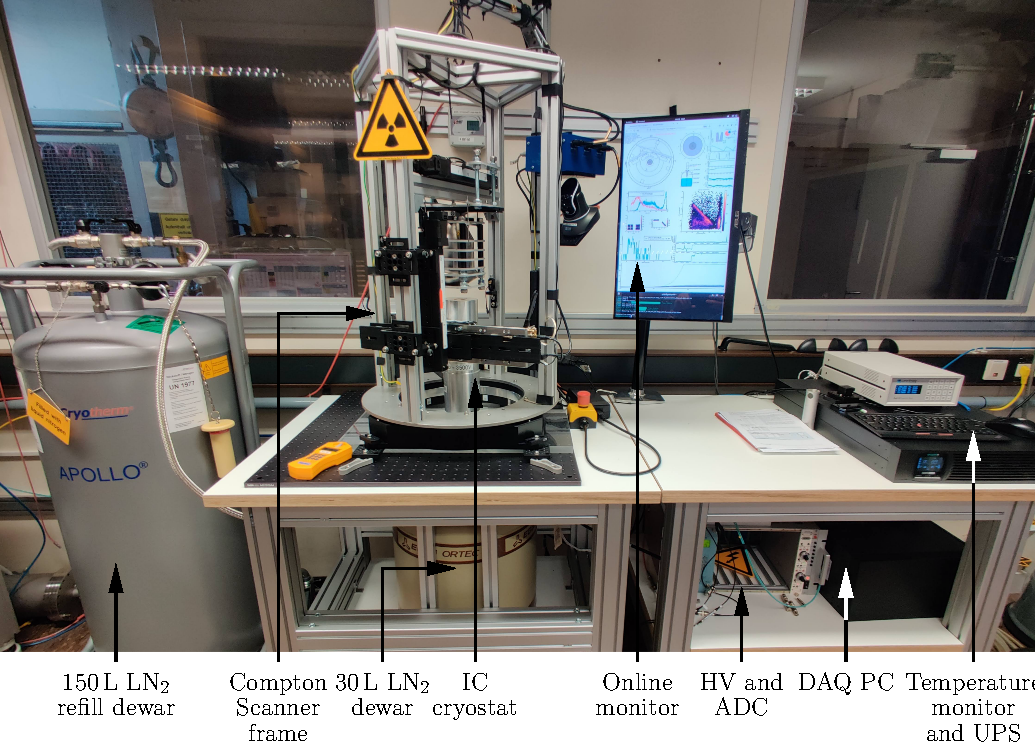
\includegraphics[width=6in]{figs/integration/full_setup_labeled_width_6_9.pdf}
    \caption{Integrated ICPC detector system with Compton Scanner frame.}
    \label{fig:full_setup}
\end{figure}

\section{ICPC Detector and its Instrumentation} \label{sec:ic_det_intru}

The geometry of the detector crystal and its contacts are shown in Fig.~\ref*{fig:ic_semiconductor} in the same orientation as in the cryostat (borehole facing dewar). The impurity concentration profile along the $\langle001\rangle$ crystallographic axis ($z$-axis in Fig.~\ref*{fig:ic_semiconductor}) was provided by the manufacturer. ORTEC used a Hall sensor to measure the impurity concentration of test slices that were cut from the regions adjacent to the top and bottom of the detector during manufacturing. The reported values at the top and bottom of the detector are $\rho_{\text{top}} = 1.109\times 10^{10}\,\text{cm}^{-3}$ and $\rho_{\text{bottom}} = 1.98\times 10^{10}\,\text{cm}^{-3}$ respectively. ORTEC recommended an operating bias voltage of 3500\,V, 550\,V over the measured depletion voltage.  
\begin{figure}[htb]
    \centering
    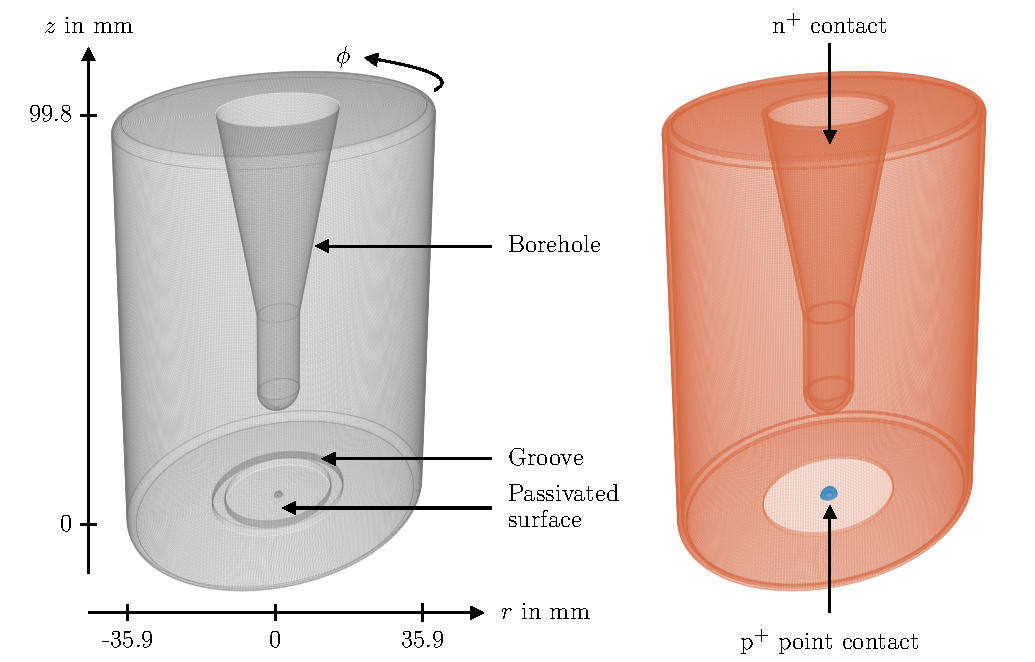
\includegraphics[width=6in]{figs/integration/P43511A_labeled_width_6_9in.pdf}
    \caption{Geometry of P43511A. The geometry of the crystal is shown in gray. The large n$^+$ contact and hemispherical p$^+$ contact on the surface of the crystal are shown in orange and blue respectively. The surface in between these contacts is passivated. Rendered with \SSD}
    \label{fig:ic_semiconductor}
\end{figure}

Upon receiving the detector at the Max Planck Institute for Physics, the four PT-100 thermoresistors were installed on the cooling rod and their cables were guided out of the dewar through the LN$_2$ vent tube shown in Fig.~\ref{fig:poptop}, before the first immersion into LN$_2$. The temperature of the detector was read out from a PopTop feedthrough connected to a MINCO-500 thermoresistor at the junction between the cooling rod and detector (see ``Temperature sensor'' in Fig.~\ref{fig:poptop_cicuit}). It was determined to be at a constant $(95 \pm 1)$\,K within a three-day LN$_2$ refill cycle and was checked periodically while data were not being taken - no deviations from this range were found.
\begin{figure}[htb]
    \centering
    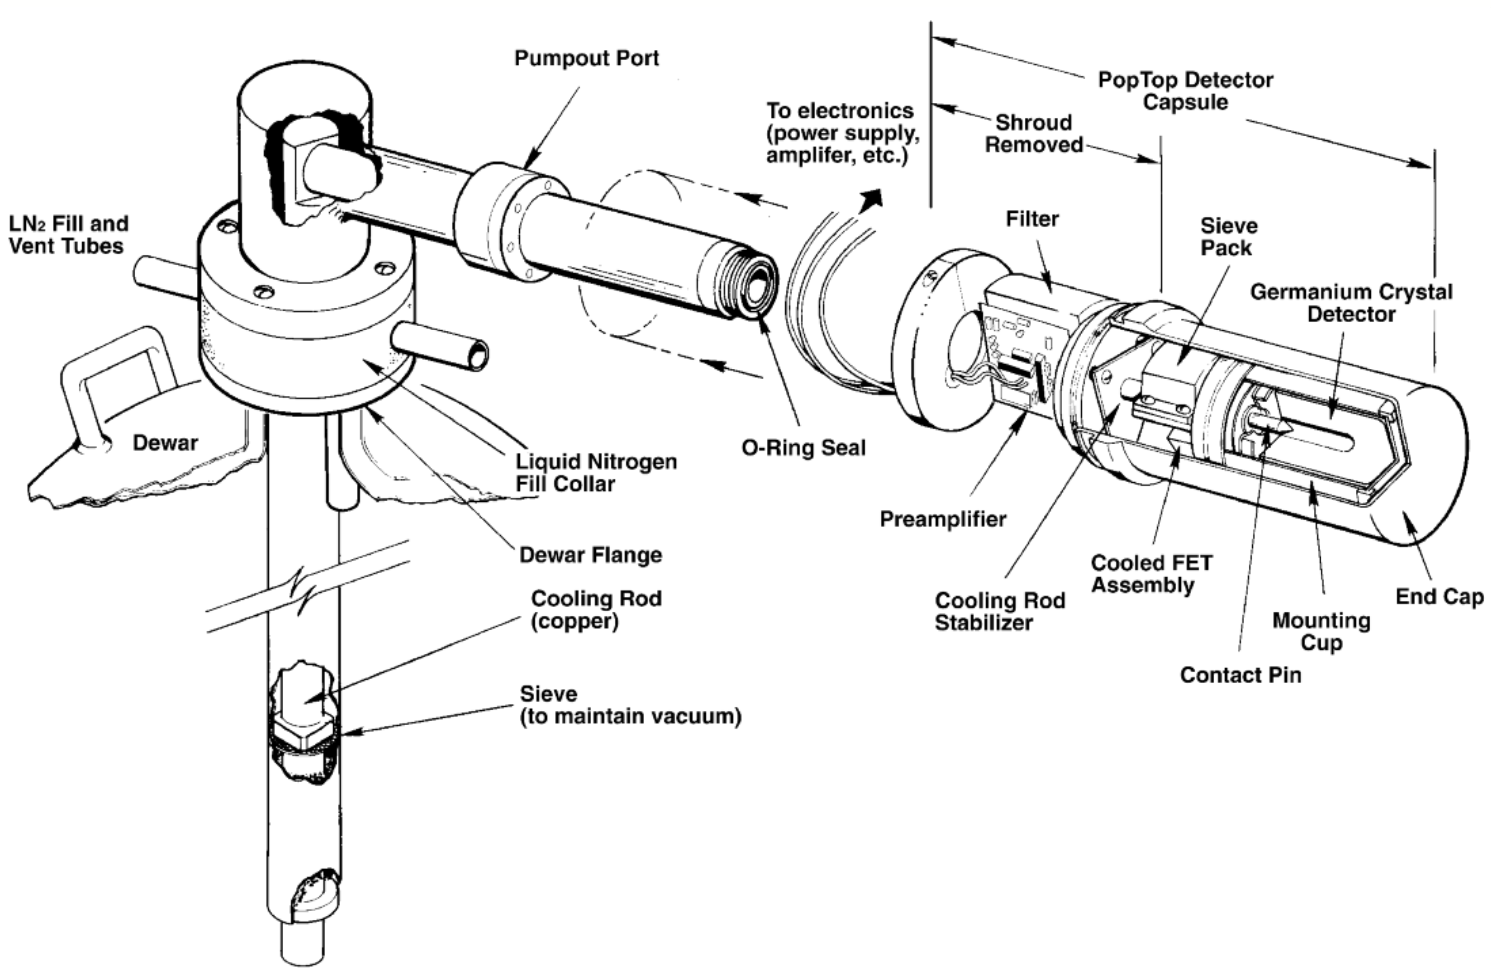
\includegraphics[width=6in]{figs/integration/poptop_labeled.png}
    \caption{PopTop cryostat with attached cooling rod and dewar in horizontal configuration. Note that this system was used in the Compton Scanner frame in vertical configuration, i.e. the cooling rod is linear and not L-shaped as shown in this diagram, and thus the detector is centered and stacked on top the collar of the dewar~\cite{poptopmanual}.}
    \label{fig:poptop}
\end{figure}

\begin{figure}[htb]
    \centering
    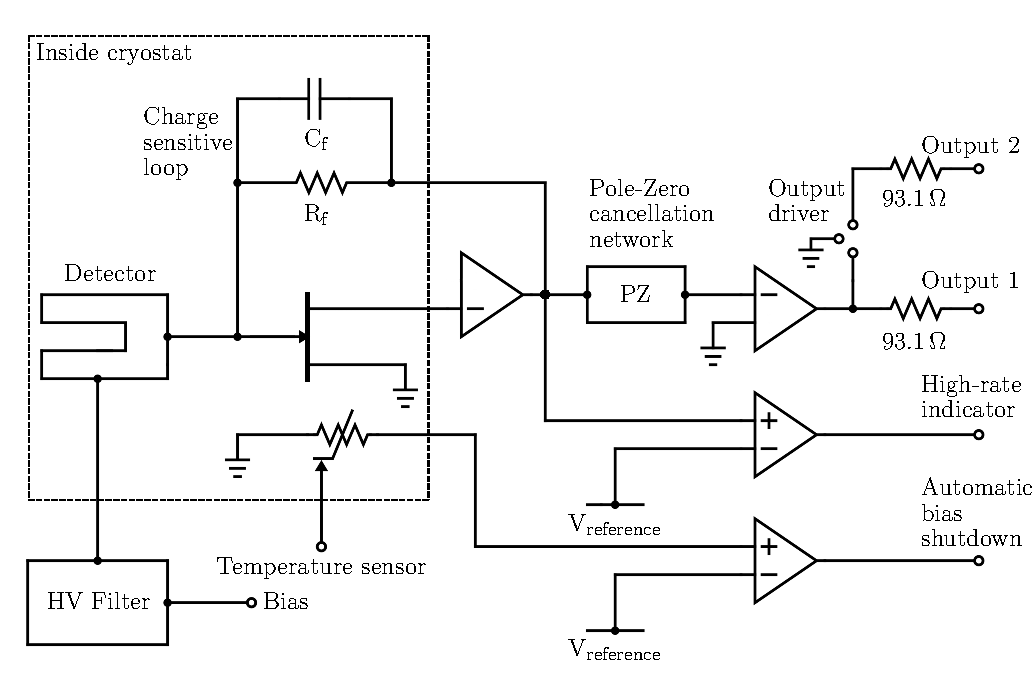
\includegraphics[width=6in]{figs/integration/poptop_circuit_width_6_9in.pdf}
    \caption{PopTop cryostat circuit level diagram. Re-rendered from the GAMMA-X\textsuperscript{\tiny\textregistered} HPGe (High-Purity Germanium) Coaxial Photon Detector System manual~\cite{poptopmanual}}
    \label{fig:poptop_cicuit}
\end{figure}


The charges induced on the point-contact of the ICPC were amplified with an ORTEC charge sensitive preamplifier as shown at the circuit level in Fig.~\ref{fig:poptop_cicuit} and its placement relative to the detector in Fig.~\ref{fig:poptop}. The preamplifier was powered by an ORTEC NIM LV supply. The circuit was placed in ``Normal mode'' (as opposed to ``Differential mode'') and thus only the signal from Output 1 is readout.  The Output 1 signals were recorded using a 14-bit ADC (STRUCK SIS3316-250-14~\cite{STRUCK}), with a sampling frequency of 250\,MHz, resulting in 4\,ns samples.

HV was applied to the ICPC at the ``Bias'' input of Fig.~\ref{fig:poptop_cicuit} with a NHQ-226 dual-channel NIM HV supply~\cite{hvsupply}. The module is controlled remotely via its RS232 serial interface which is connected to the same NetCom serial server as the motor control system (Section~\ref{subsec:motorcontrol}) and LAKE SHORE temperature monitor. The \juliapackage{Sockets} module of the standard \julia{} library was used to communicate with the serial server. Once the bias voltage was set, fluctuations of up to 0.1\,V were observed. However, the HV supply automatically ramped down on many occasions (usually once per month, with frequency increasing towards the end of operation). HV discharges are suspected to be the cause of such automatic ramp downs.

%The automatic bias shutdown circuit was determined to be faulty and was not used. Therefore the HV cannot automatically ramp down if the detector looses cryogenic temperatures, thus a strict LN$_2$ refill schedule was observed and the LN$_2$ level in the main dewar was monitored constantly. 

%The serial commands and code-snippets necessary to control and read out the HV supply (and read out temperatures from the tempreature monitor) were previously written by Lukas Hauertmann and were incorporated into the Compton Scanner control and monitoring code.


\section{Data Acquisition}\label{sec:daq}

The data acquisition settings are set in a \textit{config.scala} file which is loaded into the STRUCK ADC. This file sets parameters such as channel readout, thresholds, online energy calculation, and the length of recorded traces. These parameters were chosen depending on the measurement performed. All measurements fall into one of four DAQ modes: Germanium, Compton, Hybrid, and Noise Characterization. 
\begin{table}[tbph]
    \centering
    \caption{DAQ Modes and their settings}\label{tab:daqmodes}
	\vspace{12pt}
    \begin{tabularx}{1\textwidth}{>{\tr}X >{\tr}X >{\tr}X >{\tr}X >{\tr}X}
		\hline \noalign{\vskip 1ex}
        DAQ Mode & Trace samples ($N_s$) & Threshold & Camera status & Coincidence filtering\\[1ex]
		\hline \noalign{\vskip 1ex}
		Compton & 5000 & 100 keV & ON & Active \\
		Hybrid & 5000 &  30 keV & ON & Inactive\\
        Noise & 65532 & 0 keV & ON/OFF & Inactive\\
		\multicolumn{5}{l}{Germanium} \\[1ex]
        \quad \BaS & 5000 &  30 keV & OFF & Inactive\\
		\quad \ThS & 5000 & 100 keV & OFF & Inactive\\
		\quad \CsS & 5000 & 100 keV & OFF & Inactive\\[1ex]
		\hline
    \end{tabularx}
\end{table}

In Germanium mode, only the ICPC data is of interest and therefore the Compton Scanner was not used. \BaS{} and \ThS{} data were taken with the \CsS{} source placed as far way from the detector as its track would permit, allowing for approximately 80\,mm between the collimator borehole and the edge of the detector in the $xy$-plane. The camera system was powered off in this configuration and only Output 1 from the detector was physically connected to the ADC to minimize noise. The threshold was set depending on the type of source used, in particular it was lowered to capture the 81\,keV line of \BaS{}. Note that the detector was only scanned with the \BaS{} source illuminating from the side. In this region the 0.5-1.0\,mm thick dead layer of the n$^+$ contact stops gammas from the 31\,keV line, which have an attenuation length of approximately 0.15\,mm~\cite{NIST}. 

In Compton mode, all Compton Scanner systems were operational and only events coincident in the detector and the camera system were targeted. The only source used in this mode was \CsS{}. As Section~\ref{subsec:camera} describes, the camera readout software is proprietary. Camera data is streamed over Ethernet to the DAQ PC and thus this system is fully independent of the germanium-ADC readout. Germanium and camera data are taken in parallel. To synchronize these data streams a sync line from each camera was connected to the ADC and sync pulses were sent every 2\,s. The resulting ADC trigger times were then used to time-align the data streams. Note that sync-pulse traces were also recorded. A 3.6\,kHz event rate was observed when the \CsS{} source was driven over the detector - except over the detector borehole where the rate decreases as expected. The corresponding data rate of 2\,GB/min, made it prohibitive to keep all the recorded data; therefore a filtering script, which ran in parallel to the germanium and camera DAQ systems, used the sync pulses to select camera and germanium events which fell within a 50\,$\upmu$s coincidence window: 
\begin{equation}
	\left|t_{_{\text{IC}}} - t_{_{\text{CAM}}}\right| < 50\,\upmu s
	\label{eq:coincidence_window}
\end{equation}

Where $t_{_{\text{IC}}}$ and $t_{_{\text{CAM}}}$ are the time-aligned event time stamps of the ICPC and the camera respectively. All other data were discarded, resulting in at least a factor of 10 data reduction. The 50\,$\upmu$s coincidence window is conservative - regardless of the synchronization technique used. Most coincident event candidates fell withing a 10\,$\upmu$s time window. 

Hybrid mode was used for alignment measurements, where all events in the camera and detector, not just coincident events, were of interest. These measurements are discussed at length in Section~\ref{sec:centeralignment} and Section~\ref{sec:detcamalignment}.

In Noise Characterization mode, only the noise in the ICPC traces is of interest. Therefore, the \CsS{} source is placed in the same location as in \BaS{}/\ThS{} Germanium mode and the threshold is reduced to a minimum to only trigger on noise. The trace length is set at the maximum to observe low frequency noise since it can degrade energy resolution. This mode is intended to characterize the noise in the ICPC traces while in Germanium and Compton hardware configurations as in Section~\ref*{sec:noise}.

The \julia{} package \juliapackage{StruckVMEDevices}~\cite{struckvme}, was used to interface with the STRUCK ADC. Therefore, as with motor, HV, and temperature monitor interfaces, data can be taken directly from the \julia{} terminal. When using this package in its original form, dead times of up to 45\% were observed. Therefore, a minor modification of the code was needed. After modification, the maximum dead time was 4\%.  

In all DAQ modes 2000 samples before each trigger are recorded, ensuring sufficient statistics for baseline removal and soft pileup flagging, offline event-onset determination and energy estimation.   

\section{ICPC Center Alignment and Drift}\label{sec:centeralignment}
To accurately reconstruct event positions in the ICPC, the Compton scanner's motor coordinates -- which set the position of the camera system and the \CsS{} source --  were converted into detector coordinates. This is most easily achieved when the ICPC and Compton scanner frame are concentric, thus aligning the horizontal motor track with the radial axis of the ICPC at all rotational motor angles, $\mathcal{A}$. In practice deviations between centers always existed, and given the small vibrations introduced by motor operation and LN fills, the centers drifted over time. The geometry resulting from the non-concentric operation condition is depicted in Fig.~\ref{fig:misalignment}.
\begin{figure}[htb]
    \centering
    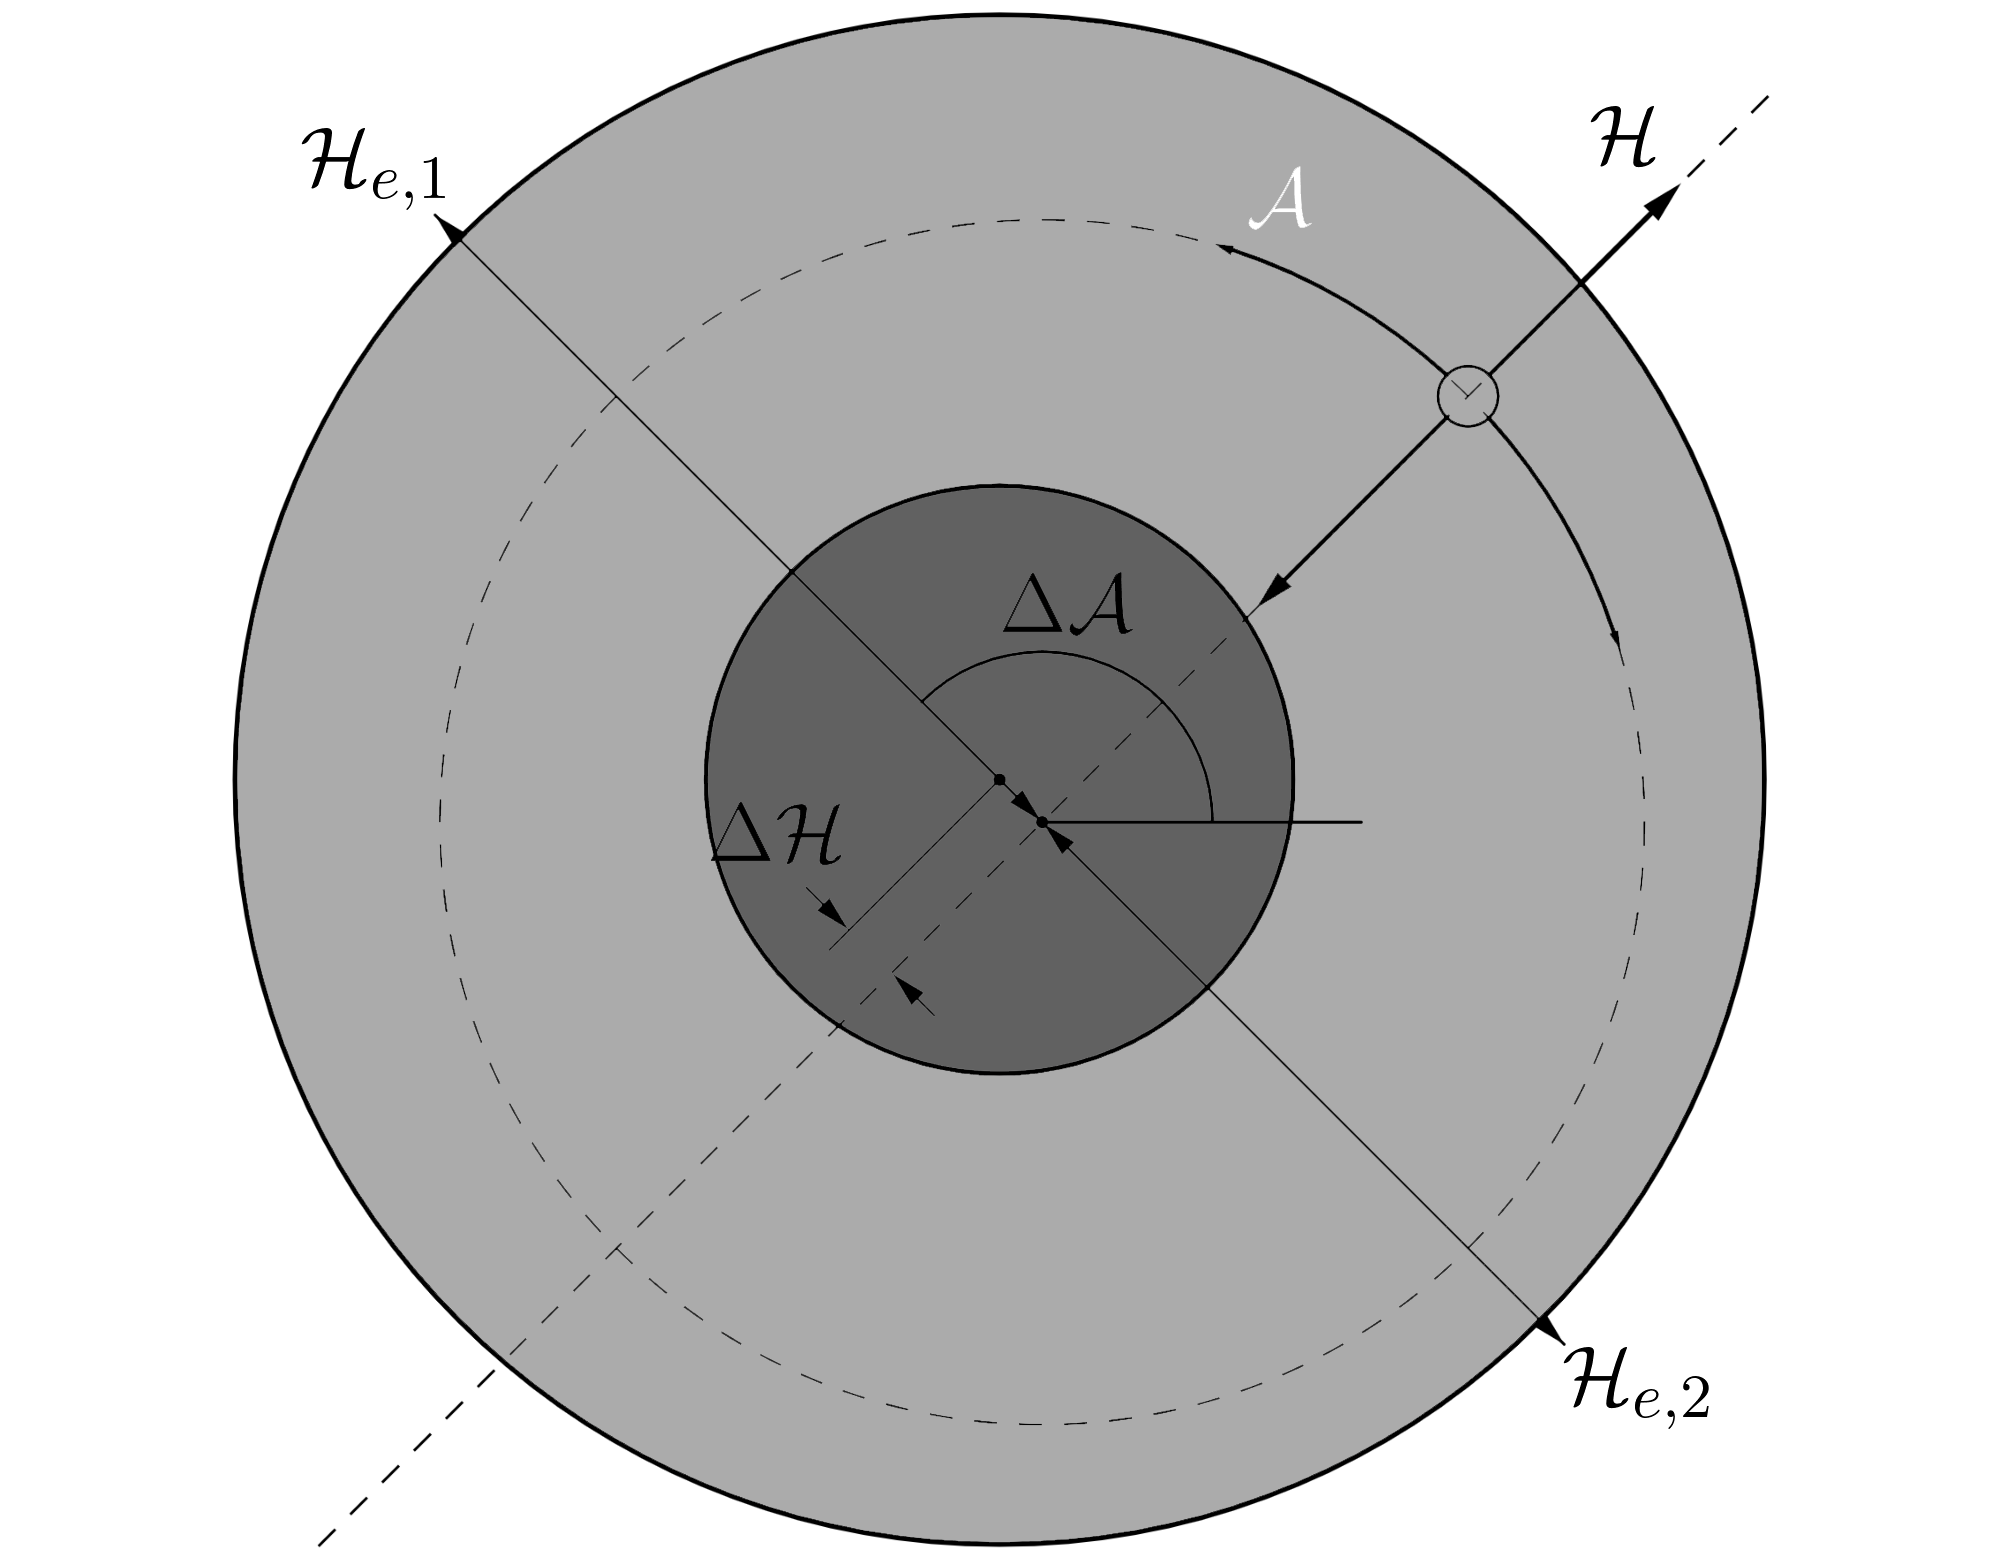
\includegraphics[width=4in]{figs/integration/icpc_alignment_quantities_labeled_width_4in.png}
    \caption{The center misalignment parameters, as defined in the text, are shown. The shaded gray areas depict the ICPC, with the borehole in dark gray. The Compton scanner frame rotational position is depicted with a dashed circle.}
    \label{fig:misalignment}
\end{figure}

As shown in the figure, the horizontal motor track, with coordinate $\mathcal{H}$, deviates from the ICPC center by $\Delta \mathcal{H}$ (in the ICPC radial direction) at rotational motor position $\Delta \mathcal{A} - 90^\circ$. The detector edges are denoted by $\mathcal{H}_e$. To determine $\Delta \mathcal{H}$ and $\Delta \mathcal{A}$, $\mathcal{H}_e$ was estimated at various angles during center alignment campaigns.

To perform the initial center alignment, and to subsequently monitor any drift from this alignment, the ICPC was scanned over a radial range -- centered at the estimated location of the detector edge -- every $\mathcal{A} = 10^{\circ} - 15^{\circ}$. The event rates at each $\mathcal{A}$ are fit to Eq.~\ref{eq:edge_fit} to compute the edge location:
\begin{equation}
    N(\mathcal{H}) = \dfrac{N_0}{2} \left[ 1 + \text{erf}\left(\dfrac{\sqrt{2} (\mathcal{H} - \mathcal{H}_e(\mathcal{A}))}{R_{eff}}\right) \right] + N_\text{B},
	\label{eq:edge_fit}
\end{equation}
where $N(\mathcal{H})$ is the event rate at each horizontal motor position, $\mathcal{H}$, and $N_0$, $N_\text{B}$, $\mathcal{H}_e$ and $R_\text{eff}$ are the floating fit parameters corresponding to the background-subtracted event rate when the \CsS{} beam is fully on the ICPC, the background event rate, the detector edge and the effective radius of the beam. This radius results from combining the effects the ICPC n$^+$ dead layer and the Gaussian profile of the \CsS{} beam. The edge fits result in $(\mathcal{A}, \mathcal{H}_e)$ pairs, which were then fit to Eq.~\ref{eq:misalignment_fit}: 
\begin{equation}
	\mathcal{H}_e(\mathcal{A}) = \mathcal{H}_0 - \Delta \mathcal{H} \cos(\mathcal{A} - \Delta\mathcal{A}) \pm \sqrt{R^2 - (\Delta \mathcal{H})^2 \sin^2(\mathcal{A} - \Delta\mathcal{A})}~,
	\label{eq:misalignment_fit}
\end{equation}
where $R$ is the active radius of the ICPC and $\mathcal{H}_0$ is the horizontal motor position of the center of the ICPC when $\mathcal{A} = \Delta \mathcal{A}$. Assuming a 1\,mm n$^+$ dead layer, $R = 34.9$\,mm. The form of the misalignment fit (Eq.~\ref{eq:misalignment_fit}) can be derived from the geometry in Fig.~\ref{fig:misalignment}. 
\begin{figure}[htb]
    \centering
    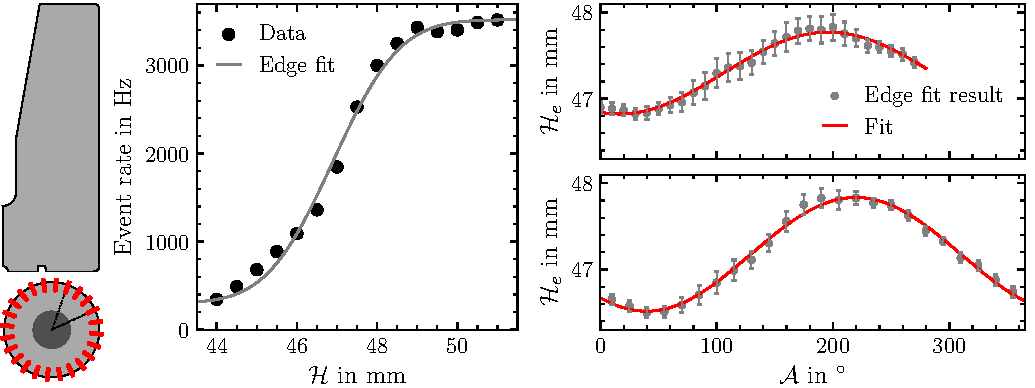
\includegraphics[width=6in]{figs/integration/center_alignment.pdf}
    \caption{The location of the edge of the ICPC ($\mathcal{H}_e$) is estimated as described in the text and exemplified for $\mathcal{A} = 0^{\circ}$ in the data panel on the left. The process is repeated for all $\mathcal{A}$'s to produce the plots on the right. The edge extracted from the fit at each $\mathcal{A}$ is shown for the 2022-03-21 and 2022-09-05 calibrations in the top and bottom respectively. In the far left, a pictogram depicts a radial slice of the ICPC and a top view. The top view shows the \CsS{} source positions for the 2022-09-05 alignment.}
    \label{fig:center_alignment}
\end{figure}

Before the beginning of the main data taking campaign, a near-concentric condition was achieved by iteratively moving the Compton scanner frame with respect to the ICPC and performing center alignment scans and fits. In this process, it was concluded that motor operation and LN refills did not significantly alter the alignment. The best possible alignment was achieved on 2022-03-21, from which point the integrated system was not re-aligned. On 2022-06-20 and 2022-09-05 center alignment scan were performed, where the latter was taken close to the end of ICPC operations. Fig.~\ref{fig:center_alignment} depicts the edge fitting procedure, as well as the misalignment fits for the initial and final scans. The misalignment quantities deduced from the fits are summarized in Tab.~\ref{tab:misalignment}.
\begin{table}[tbph]
    \centering
    \caption{Summary of misalignment quantities derived from the three center alignment scans.}
	\vspace{12pt}
	\begin{tabularx}{1\textwidth}{>{\tr}X >{\tr}X >{\tr}X >{\tr}X}
		\hline \noalign{\vskip 1ex}
		Date & $\mathcal{H}_0$ in mm & $\Delta \mathcal{H}$ in mm& $\Delta \mathcal{A}$ in $^\circ$\\
		\hline \noalign{\vskip 1ex}
		2022-03-21 & $82.20 \pm 0.01$ & $0.47 \pm 0.01$ & $16.2 \pm 1.7$\\
		2022-06-20 & $82.15 \pm 0.01$ & $0.45 \pm 0.01$ & $28.5 \pm 1.9$\\
		2022-09-05 & $82.07 \pm 0.01$ & $0.66 \pm 0.01$ & $39.7 \pm 1.2$\\[1ex]
		\hline
	\end{tabularx}
	\label{tab:misalignment}
\end{table}

Although less accurate, scans across the full detector also estimate an ICPC center location of approximately 82\,mm, supporting the 1\,mm-dead-layer assumption, and the misalignment fits. It is clear that near concentric conditions were maintained during the main data taking campaign. Thus, in this work, the following concentric coordinate approximation is used to transform motor to detector coordinates $(r,\phi,z)$:
\begin{equation}
    r = 82\,\text{mm} - \mathcal{H},\quad \phi = \mathcal{A}
\end{equation}
If needed, the exact coordinate transformation can be performed as follows, using the most relevant misalignment quantities from Tab.~\ref{tab:misalignment}:
\begin{align}
    r &= \sqrt{\vert\mathcal{H} - \mathcal{H}_0\vert^2 + (\Delta\mathcal{H})^2 - 2 \Delta\mathcal{H} \vert\mathcal{H} - \mathcal{H}_0\vert \cos(\mathcal{A}-\Delta\mathcal{A})}, \label{eq:realr} \\ 
    \phi &= \text{asin} \left(\dfrac{\vert\mathcal{H} - \mathcal{H}_0\vert\sin(\mathcal{A} - \Delta\mathcal{A})}{r} \right) + \Delta\mathcal{A}~, \label{eq:realphi}
\end{align}

All measurements were performed in the $\|\mathcal{A} - \Delta \mathcal{A}\| < 60^\circ$ and $\|\mathcal{A} - (\Delta \mathcal{A} + 180^\circ)\| < 60^\circ$ ranges, thus in most cases the concentric approximation results in an under 2$^\circ$ deviation from the value calculated by Eq.~\ref{eq:realphi}. Only in the inner 10\,mm and far from $\Delta \mathcal{A}$ or $\Delta \mathcal{A} + 180^\circ$ is the deviation considerably larger. However, such deviations mostly fall within the angles subtended by the \CsS{} beam spot in these locations. For the entire detector, the concentric approximation results in an under 0.7\,mm deviation from the radial value calculated by Eq.~\ref{eq:realr}.

\section{ICPC - Camera Alignment} \label{sec:detcamalignment}
The hit positions in the camera data stream are given in local coordinates. Whenever camera (B) was used, its local coordinates were first transformed to the coordinate system of camera (A) as exemplified by Fig.~\ref{fig:czt_relative2D}. To perform position reconstruction, the camera coordinates were then transformed to into global coordinates, with an origin located at the bottom of the detector as shown by Fig.~\ref{fig:workingprinciple} and Fig.~\ref{fig:czt_icpc_alignment_pictures}. Note that $(x,y)$-alignment of the ICPC and camera is vital to the $z$-reconstruction, as the distance between the \CsS{} beam position and camera hit location appears in Eq.~\ref{eq:ztheta}. 

The horizontal motor track allows the \CsS{} to be placed over the camera (A). The \CsS{} beam was captured by the camera and shown in Fig.~\ref{fig:czt_icpc_alignment}. In this manner, a reference between the camera system and horizontal motor track is constructed, allowing for the calculation of the $(x,y)$-offset between the ICPC and camera (A). The marginalized beam profile (1-hit, 662\,keV events) is fit to a Gaussian in the $x$- and $y$-directions to calculate the center of the beam spot on the camera. 
\begin{figure}[htb]
    \centering
    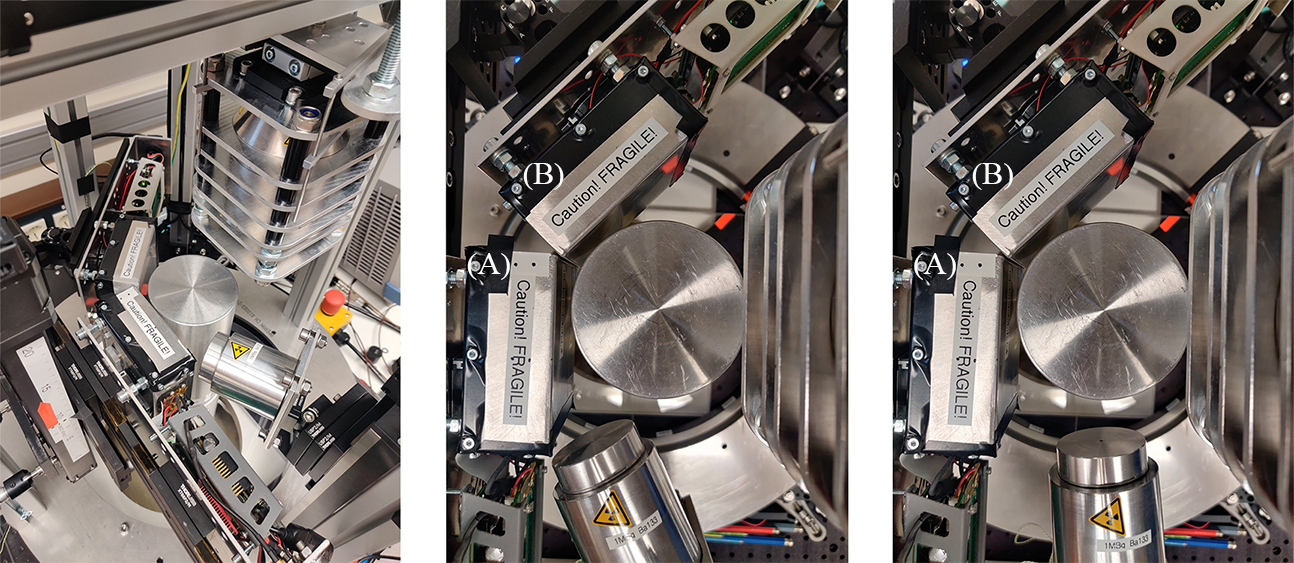
\includegraphics[width=6in]{figs/integration/czt_icpc_alignment_pictures_labeled.png}
    \caption{The ICPC-camera alignment setup is pictured, where the \CsS{} source was moved to the right as to not block the view of the setup. The \BaS{} source swings to point at camera (A) and at the ICPC (middle and right pictures respectively).}
    \label{fig:czt_icpc_alignment_pictures}
\end{figure}

A similar strategy is used for $z$-alignment. A collimated \BaS{} source was temporarily mounted on a vertical motor stage, 90$^\circ$ from camera (A). The source could swing to point at camera (A) and at the ICPC while ensuring that the beam remained perpendicular to the $z$-axis. This temporary setup is shown in Fig.~\ref{fig:czt_icpc_alignment_pictures}. 
\begin{figure}[htb]
    \centering
    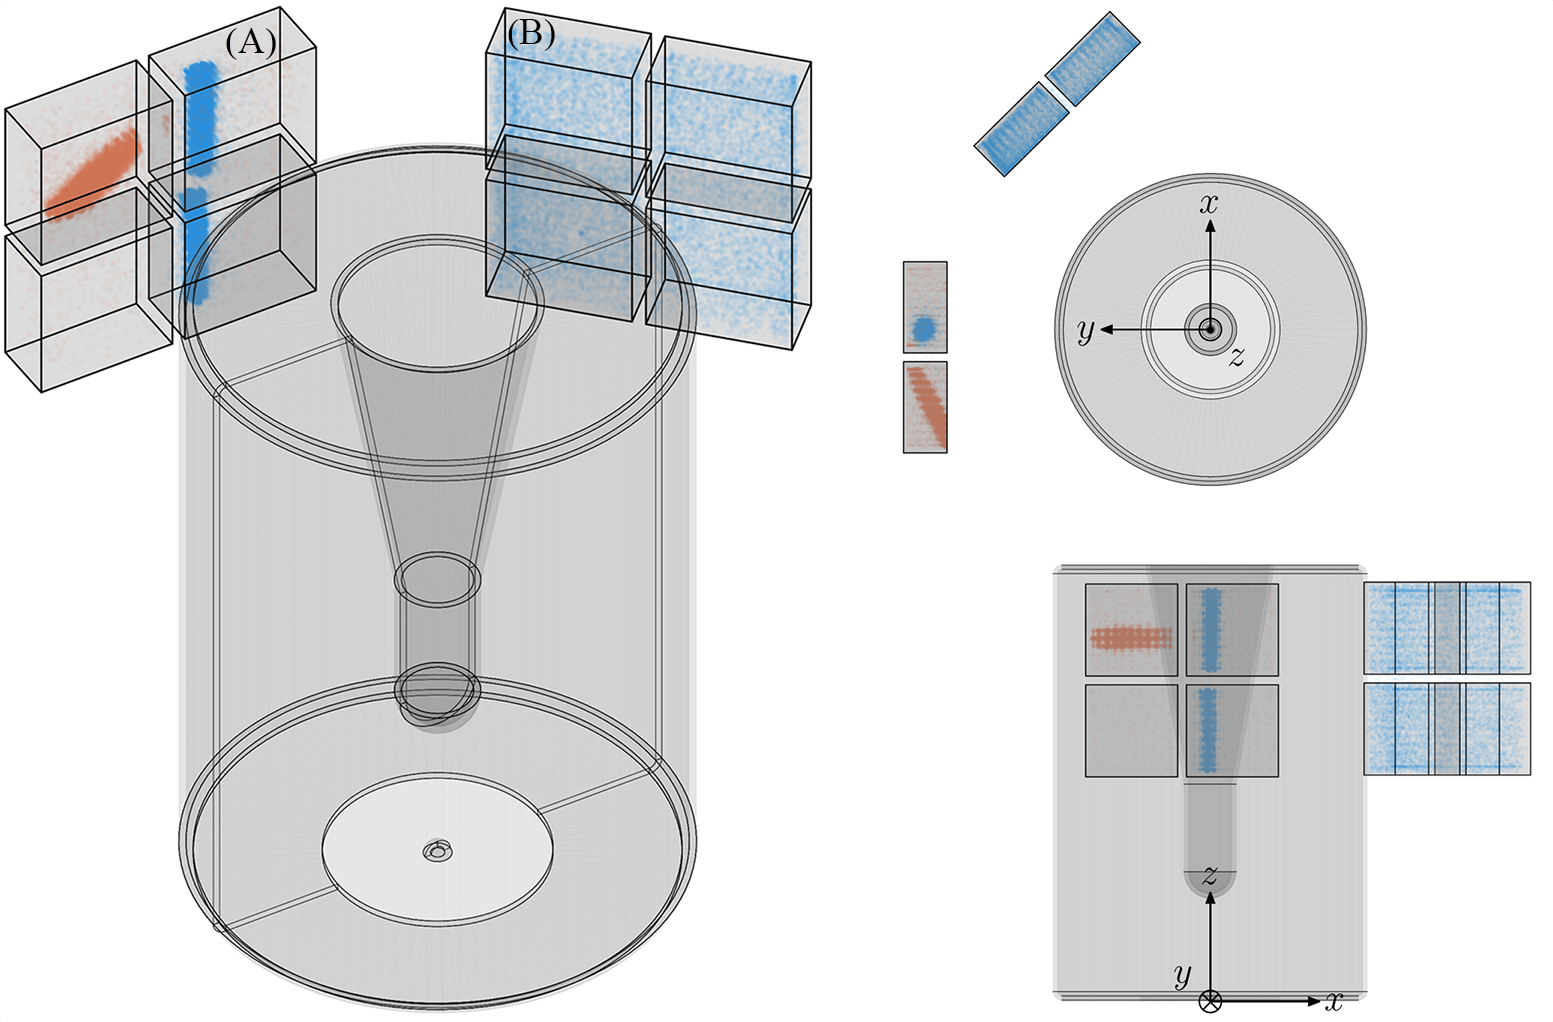
\includegraphics[width=6in]{figs/integration/czt_icpc_alignment_labeled_rq.png}
    \caption{\CsS{} and \BaS{} camera hits are shown in blue and orange respectively for the ICPC-camera alignment measurements in an isometric, top and lateral view of the integrated system. The later two views also feature the global coordinate system used. The sources were pointed in turn at camera (A), but the resulting hits are shown together for convenience. Camera (A) depicts \CsS{} 1-hit, 662\,keV events and \BaS{} 1-hit, 81\,keV and 356\,keV events. On the other hand, camera (B) shows all events from the \CsS{} measurement, predominantly Compton scatters from camera (A) and the surrounding structures. All components are rendered to scale.}  
    \label{fig:czt_icpc_alignment}
\end{figure}

A reference $z$-value was obtained by pointing the \BaS{} source to camera (A) and fitting $z$-profile of the beam (1-hit, 81\,keV and 356\,keV events) to a Gaussian. The \BaS{} source was also pointed at the ICPC, where an edge scan and fit (using the same techniques described in the last section) were performed to locate the top edge of the ICPC. In this manner the $z$-offset between the ICPC was and camera was found. Note that the camera is also on a vertical motor stage, thus a difference in camera motor positions is added to the $z$-offset when the camera is moved vertically from the position in which the alignment was performed. The \BaS{} beam was captured by the camera and shown in Fig.~\ref{fig:czt_icpc_alignment}.

In principle, the $z$-alignment is not needed, which is one of the advantages of the Compton reconstruction technique: the reconstructed $z$-position is simply offset by the $z$-position of the origin of the system of coordinates. However, performing this alignment had a twofold benefit. First it allowed for the camera to be optimally placed (before reconstruction) to target specific regions in the detector. Second, once reconstruction was performed, it served as a cross-check: giving the rage of $z$-values in which the reconstructed events should lie. 


\section{Noise} \label{sec:noise}
Test data were taken with the integrated the ICPC-Compton Scanner system in Compton and Germanium DAQ modes. A systematic analysis of data quality revealed large noise bursts in the waveforms collected in both DAQ modes. Two such events are plotted in Fig.~\ref{fig:burst_waveforms}. 
\begin{figure}[htb]
    \centering
	\vspace*{-10pt}
    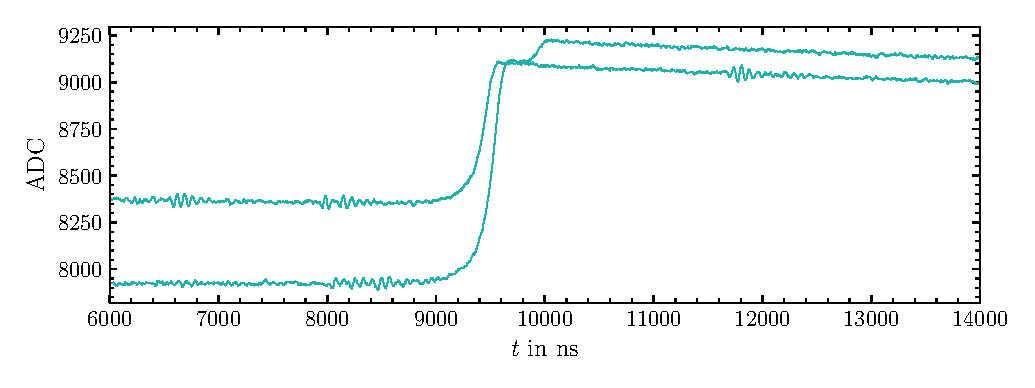
\includegraphics[width=6in]{figs/param/burst_waveforms_6_9in.pdf}
	\vspace*{-10mm}
    \caption{Two waveforms exhibiting noise bursts in Compton DAQ mode. A burst obscures the beginning of the rise of the waveform on the bottom.}
    \label{fig:burst_waveforms}
	\vspace*{-5pt}
\end{figure}

The presence of bursts is not expected to deteriorate the energy resolution significantly, since the energy estimator (see trapezoidal shaping times in Section~\ref{sec:energy}) averages over a window many times longer than the period of the oscillations within a burst. However, the parameters calculated from pulse shape, such as the onset of the rise, $t_{0}$, are significantly impacted by the presence of bursts on the rising edge. The long traces taken in Germanium Noise Characterization mode (cameras off) reveal that bursts come in packets lasting longer than the maximum 262\,$\upmu$s recording time of the ADC. A burst frequency of 30\,kHz within a packet is determined from events like the one traced in Fig. \ref{fig:long_trace}. Each burst consists of two sub-bursts with an oscillation frequency of 11\,MHz and a separation of about 2\,$\upmu$s between centers. The estimated average amplitude of each burst is 42\,ADC units. Such an amplitude corresponds to roughly a quarter of that reached by a \BaS{} 81\,keV gamma event. 
\begin{figure}[htb]
    \centering
	\vspace*{-10pt}
    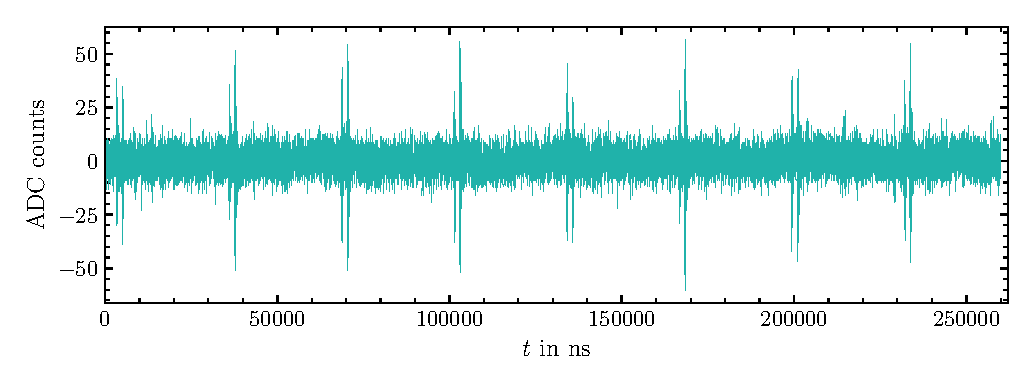
\includegraphics[width=6in]{figs/param/long_trace_width_6_9in.pdf}
	\vspace*{-10mm}
    \caption{A baseline subtracted event taken in Germanium Noise Characterization mode.}
    \label{fig:long_trace}
	\vspace*{-5pt}
\end{figure} 

To optimize data quality it is evident that events with noise bursts on or close to the rising edge of a waveform should be removed. Given that the event triggers are independent of the onset of bursts, the number of bursts at the rising edge can be estimated from any window of the same duration. The natural choice is to use the baseline. The baseline width, $B_w(N_s)$, defined as the difference between the maximum and minimum ADC value of the first $N_s$ samples in a waveform, is used to estimate the prevalence of noise burst events. From simulation (Section~\ref{sec:ic_sims}), the maximum drift time in the ICPC is approximately 2.2\,$\upmu$s, therefore a conservative window of $N_s = 1000$ samples (4\,$\upmu$s) is set for the rising edge. The $B_w(1000)$ distributions of test data taken in Compton and Germanium DAQ modes are shown in Fig.~\ref{fig:baseline_width_pre_optical}. Note that events with pileup were removed from both data sets using a technique that will be described in Section~\ref{sec:pileup}. 
\begin{figure}[htb]
    \centering
	\vspace*{-10pt}
    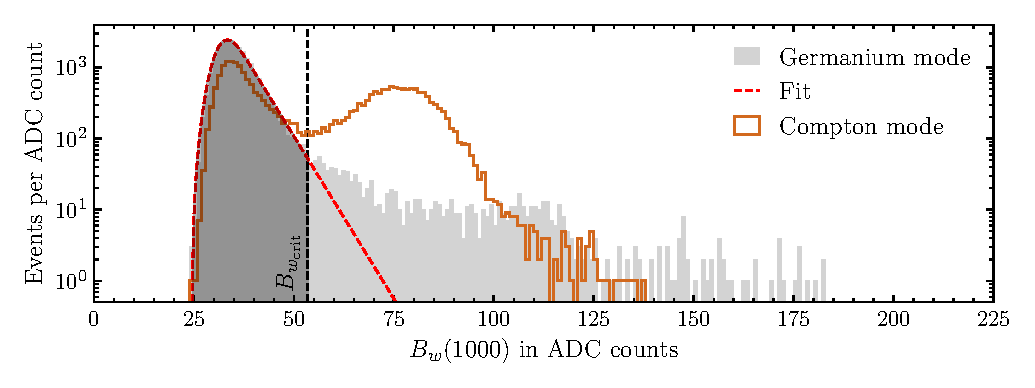
\includegraphics[width=6in]{figs/param/baseline_width_pre_optical_6_9in.pdf}
	\vspace*{-10mm}
    \caption{Baseline width distribution of $2.5\times10^4$ events taken in Compton DAQ mode and Germanium DAQ mode. Compton mode noise bursts are evident in the second peak in brown, centered around $B_w(1000) = 84\,\text{ADC}$. Baseline width of Germanium mode noise characterization data is fit to the high-energy-tail version of the response function of Eq.~\ref{eq:energy_peak_fit}.}
    \label{fig:baseline_width_pre_optical}
	\vspace*{-5pt}
\end{figure}

The overwhelming presence of burst events in Compton mode creates a clear separation between burst events and burst-free events in the $B_w(1000)$ distribution. Germanium mode test data is used to estimate $B_w(1000)$ for a population of burst-free events.  The main peak is fit to the same response function used for energy peaks (Gaussian plus exponentially modified Gaussian tail -- Eq.~\ref{eq:energy_peak_fit}), but with modifications to switch from a low-end to a high-end tail. A cut is set at the value where 99\% of the area under the fitted peak is covered. Events with $B_w(1000) > B_{w_\text{crit}}  = 53$\,ADC are chosen as burst event candidates. The resulting burst contamination in a 1000 sample window is 49\% and 4.6\% in Compton mode and Germanium mode test data respectively. It is clear that the camera system was introducing unacceptable amounts of noise into ICPC data. Steps were thus taken to isolate the camera system from the ICPC in hopes of matching the Germanium mode performance.

\section{Optical Isolation}
Germanium mode performance was optimized using $B_w(1000)$ as a figure of merit, prior to camera-ICPC isolation. Lower modes of the $B_w(1000)$ distribution indicate lower overall noise amplitude, while significant high-value tailing or secondary peaks indicate noise bursts. With this in mind, data were taken in dozens of grounding and power configurations. This campaign led to the final configuration of the system, which minimized, but did not fully eliminate the presence of bursts and lowered the overall noise amplitude. An overview of this configuration follows
\begin{enumerate}
	\item The ADC was coupled to the DAQ PC directly with fiber optics. This eliminated a ground loop created by the ADC-Ethernet-Switch copper connections. Note that camera system needs to be connected to this Ethernet Switch. 
	\item All systems were powered from the same UPS except the ADC. When the camera system was put into operation, the best performance was achieved when it was powered from a different source than the ADC and the UPS. 
	\item All large metal components surrounding the ICPC cryostat were grounded to the same ground of the UPS. This includes the Compton Scanner frame, aluminum breadboard, and camera enclosures.  
\end{enumerate} 

Reintegration of the camera system was investigated with the new integrated hardware configuration. Once again, when cameras were turned on, the prevalence of bursts increased. However, a significant reduction of bursts was observed when the sync copper cables of both cameras were disconnected from the ADC, an effect that had not been observed previous to the grounding and cabling changes. Due to hardware limitations, sync pulses could not be sent over optical fibers, however optical isolation can still be achieved by placing a IL300 optocouple~\cite{il300} in each camera copper sync line as Fig.~\ref{fig:optocoupler} shows.   
\begin{figure}[htb]
    \centering
	\vspace*{-10pt}
    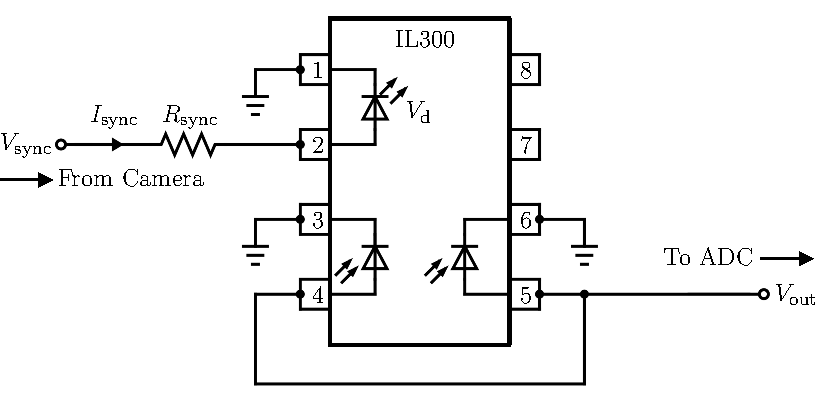
\includegraphics[width=5.5in]{figs/param/optocoupler_circuit_width_5_5in.pdf}
    \caption{The IL300 integrated circuit~\cite{il300} is placed in the sync line from each camera to the ADC to send sync pulses without a copper connection.}
    \label{fig:optocoupler}
	\vspace*{-5pt}
\end{figure}

Each camera outputs a $V_{\text{sync}} = 3.3$\,V sync pulse.  The sync pulse length was set to match the switching time of IL300: 1\,$\upmu$s. The duration of the pulse was originally set to 50\,ns, resulting in the copper sync pulse shown in Fig.~\ref{fig:sync_pulses}. The resistance on the camera sync line, $R_{\text{sync}} = 100\,\Omega$, was chosen to drive the infrared LED in IL300 ($V_\text{d} = 1.25$\,V) with a current of $I_{sync} = (V_{\text{sync}} - V_\text{d})/R_{\text{sync}} \approx 20$\,mA, to not draw too much current from the camera. This current is sufficient to drive the LED in its optimal range~\cite{il300}. The two photodiodes in IL300 are operated in photovoltaic mode and their output is recorded by the ADC. $V_{\text{out}} \approx 5$\,mV is estimated from the amplitude of resulting optical sync pulses such as that in Fig.~\ref{fig:sync_pulses}.
\begin{figure}[htb]
	\centering
	\vspace*{-10pt}
    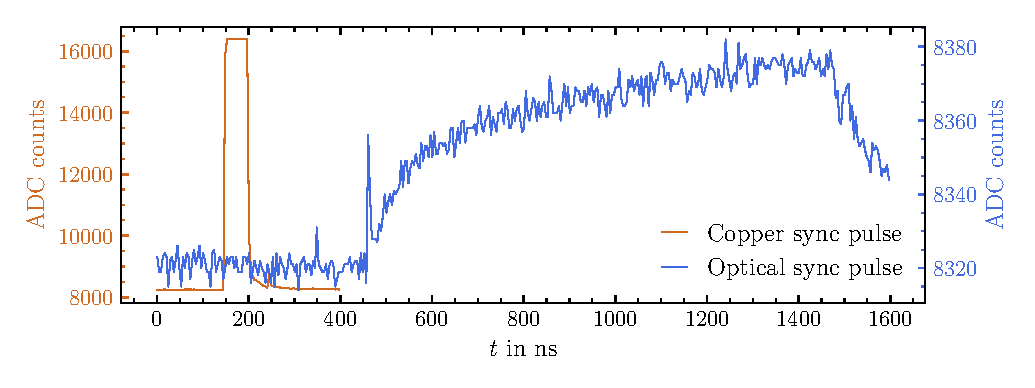
\includegraphics[width=6in]{figs/param/sync_pulses_width_6_9in.pdf}
	\vspace*{-10mm}
	\caption{A 50\,ns, 3.3\,V sync pulse saturates the ADC with a direct copper connection. In the same frame, but with different $y$-scale, the optocoupler response to a 1\,$\upmu$s, 3.3 V sync pulse is shown.} 
	\label{fig:sync_pulses}
\end{figure}
The vastly different rise times of the copper and optical sync pulses can be seen from their scales in Fig.~\ref{fig:sync_pulses}.  Nevertheless, the coincidence window is 50 times wider than the 1\,$\upmu$s risetime of an optical sync pulse. Thus, it is expected that the longer risetimes of the optical sync pulses does not significantly affect the number of events falling within the coincidence window. This becomes evident from the distribution of $t_{_{\text{IC}}} - t_{_{\text{CAM}}}$ within the coincidence window shown in Fig.~\ref{fig:coincidence_window}. A 5.5\% drop in coincidence rate is found with the introduction of the IL300 optocouplers in the sync lines. 
\begin{figure}[htb]
    \centering
	\vspace*{-10pt}
    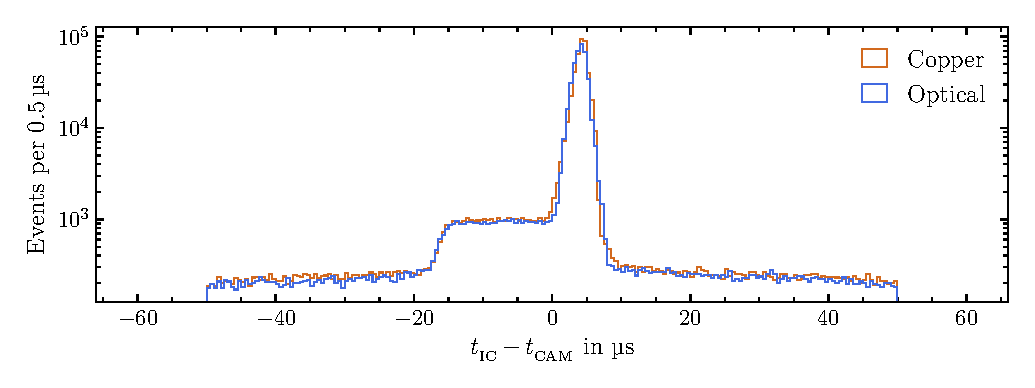
\includegraphics[width=6in]{figs/param/coincidence_window_6_9in.pdf}
	\vspace*{-10mm}
    \caption{ Distributions of $t_{_{\text{IC}}} - t_{_{\text{CAM}}}$ in the 50\,$\upmu$s coincidence window for 3100\,s of Compton mode data taken with the IL300 optocoupler placed in the sync lines (Optical) and without (Copper). The coincident event rates are 147.3\,Hz and 155.8\,Hz respectively.}
    \label{fig:coincidence_window}
	\vspace*{-5pt}
\end{figure}

The optimized Germanium and Compton hardware configurations were tested in Noise Characterization DAQ mode. Compton data were taken with the IL300 optocoupler placed in the sync lines and without, which are referred to as the optical sync and copper sync configurations, respectively. The optical sync configuration matched the noise performance that was achieved by disconnecting the sync cables from the ADC. For the optical and sync configurations, data were taken with camera (A) on and camera (B) off, and with both cameras on. Germanium mode data were taken to establish the baseline noise performance.  

%A baseline selection criterion is established by calculating the root-mean-square (RMS) of the mean ADC values of background-free population of waveforms. These events are selected from 24000 Germanium mode data events. The mean of the first 200 samples is subtracted from each waveform. Events where the mean of the next 1000 samples is $\ge0$\,ADC are selected. This automatically eliminates soft pileup. Non-baseline events are dominated by background radiation. The probability of a background event falling within an event window ($\Delta t$), given a background rate of $r$, is calculated with the Poisson distribution.
%\begin{equation} \label{eq:poisson}
	%P(n = k) = \frac{(r\Delta t)^{k}e^{-r\Delta t}}{k!}
%\end{equation}
%The probability of zero background events ($k = 0$) falling within an event window of $\Delta t = 1000 \times 4\,\text{ns}$ is 99.9\%, given the 100\,keV-threshold background rate of 302\,Hz (calculated in Section~\ref{sec:centeralignment}). Even with a conservative $10 \times$ higher background -- to account for the 0\,keV threshold that was used here -- the probability only descends to 98.6\%. Thus, the selected events are overwhelmingly baseline events within the 1000-sample window. The RMS of the means of these 1000-sample windows is then calculated (RMS$_{\mu 1000}$) and and and upper limit is set at $5\text{RMS}_{\mu 1000}$. Each waveform is then averaged in 1000 sample intervals. If the mean any interval is above $5\text{RMS}_{\mu 1000}$ the waveform is tagged as a non-baseline. This technique eliminates most soft and hard pileup events and other background events or anomalous waveforms. 76.9\% of events survive the baseline cut.

%Background radiation will either be seen as a trigger within the $\Delta t_\text{event} = 65532 \times 4\,\text{ns}$ event window or as a decaying baseline if the trigger occurs before the event window (soft pileup). The average background energy (with 100\,keV threshold) is 315\,keV which corresponds to $\text{max(ADC)} \approx 566\,\text{ADC}$. The decay constant calculated in Section~\ref{sec:electronicsresponse}, $\tau = 55.53\,\upmu$s, is used to establish the decay window of $\Delta t_\text{decay} = n_\text{decay}\tau$. A baseline is counted as restored if the 1000-sample-mean ADC value of a waveform falls below the expected value of $5\text{RMS}_{\mu 1000}$. From $\text{max(ADC)}e^{-n_\text{decay}\tau} = 5\text{RMS}_{\mu 1000}$, $n_\text{decay} = 4.9$ is extracted. Setting the probability of finding no background events within the decay window and the subsequent event window ($\Delta t = \Delta t_\text{decay} + \Delta t_\text{event}$) in Eq. \ref{eq:poisson} to the baseline cut survival probability, the true background rate can be calculated. From this, a 494.8\,Hz 0\,keV-threshold background rate is determined. Note that this corresponds to a very reasonable 1.64 times higher background rate than that with a 100\,keV threshold.

The performance of the 5 hardware configurations is characterized by taking a Fast Fourier Transform (FFT) of each waveform and then averaging the FFTs in each data set. To ensure the fidelity of the averaged FFT, FFTs are only be performed on baselines. To remove background events, an offline trigger in the form of the trapezoidal filter (with parameters equal to that of the pileup trapezoidal filter -- Sec.~\ref{sec:pileup}) was used. Events which triggered were removed from the analysis and the FFTs and $B_w(1000)$ distributions are calculated for each data set. The $B_w(1000)$ distributions of all 5 hardware configurations are shown in Fig.~\ref{fig:baseline_width_optical}. As expected Germanium mode noise amplitude is the lowest overall and exhibits the lowest prevalence of bursts. There is a clear suppression of burst abundance in data taken with optical sync lines with respect to their copper sync line counterparts. In both cases, bursts are most prevalent when both cameras are operated. Nonetheless, near-germanium-mode performance was achieved in Compton mode with optical sync lines and camera (B) off. As in Section~\ref{sec:noise}, $B_w(1000)$ for a population of ``burst-free'' events is calculated from Germanium mode data.
\begin{figure}[htb]
    \centering
	\vspace*{-10pt}
    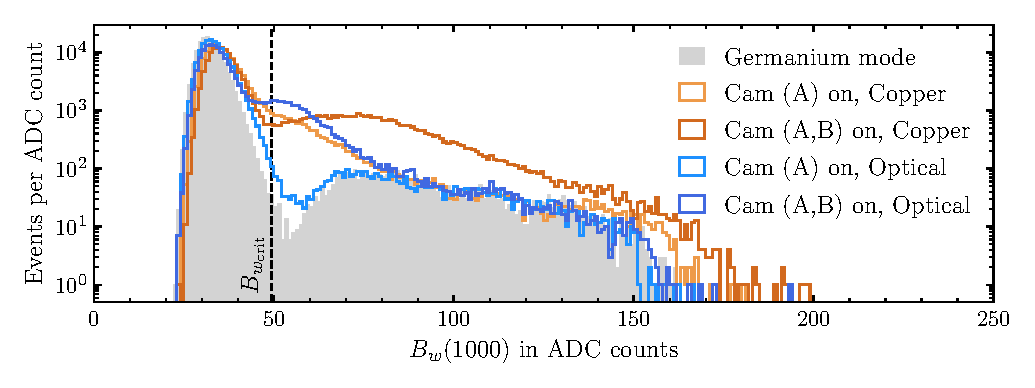
\includegraphics[width=6in]{figs/param/baseline_width_all_modes_6_9in.pdf}
	\vspace*{-10mm}
    \caption{Baseline width distribution of $1.5\times10^5$ events in all 5 hardware configurations.}
    \label{fig:baseline_width_optical}
	\vspace*{-5pt}
\end{figure}

Setting a 99.9\% fitted peak area coverage, events with $B_w(1000) > B_{w_\text{crit}}  = 49$\,ADC are chosen as burst event candidates. Note that a higher coverage of the main peak is used due to the clearer separation of burst and non-burst events in comparison to test data. Setting this cut, a lower sacrifice of non-burst events is obtained. Burst abundance is quantified from the distributions in Fig.~\ref{fig:baseline_width_optical} with the described cut value and presented in Tab.~\ref{tab:noise_results}.
\begin{table}[tbph]
	\centering
	\caption{Burst abundance in a 1000-sample window of test data and the five hardware configurations described in the text. The abundance is calculated as the fraction of events passing the $B_w(1000) \ge B^\prime_{w_\text{crit}}$ and $ B_w(1000) \ge B_{w_\text{crit}}$ cuts for test data and noise characterization data respectively.} 
		\vspace{12pt}
		\begin{tabularx}{1\textwidth}{bsss}
			\hline \noalign{\vskip 1ex}
			DAQ Mode & No sync & Copper sync & Optical sync\\[1ex]
			\hline \noalign{\vskip 1ex}
			Germanium test & 0.046 & -- & --\\
			Compton test (cam (A,B) on) & -- & 0.49 & --\\
			Noise -- Germanium & 0.026 & -- & --\\
			Noise -- Compton: Cam (A) on & -- & 0.095 & 0.027\\
			Noise -- Compton: Cam (A,B) on & -- & 0.24 & 0.15 \\[1ex]
			\hline
		\end{tabularx}
		\label{tab:noise_results}
\end{table}

A separate FFT was produced for burst-free Germanium mode data ($B_w(1000) \le B_{w_\text{crit}}$) and burst-dominant Germanium mode data ($B_w(1000) > B_{w_\text{crit}}$). To identify the signatures in the FFT for burst events. Busts can be identified by increased noise levels and large oscillations in the expected 9 - 20\,MHz range in Fig.~\ref{fig:fft_ge_log}. By comparing optical sync pulse data to copper sync pulse data in this range for both camera configurations (Fig.~\ref{fig:fft_ge}), there is a clear suppression of bursts in optical sync line data.
\begin{figure}[htb]
    \centering
	\vspace*{-10pt}
    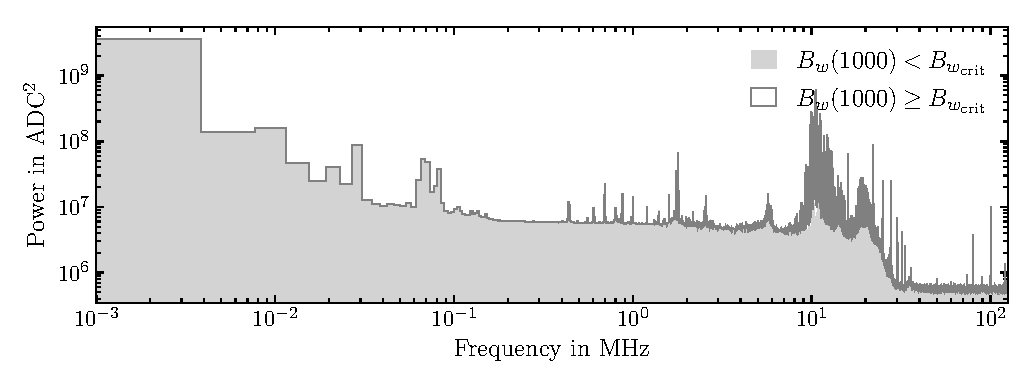
\includegraphics[width=6in]{figs/param/fft_ge_mode_log_width_6_9in.pdf}
	\vspace*{-10mm}
    \caption{FFTs of 5\,min of burst-free and burst-dominated Germanium mode data. Note that all noise characterization measurements incur an 83.8\% deadtime.}
    \label{fig:fft_ge_log}
	\vspace*{-5pt}
\end{figure}

\begin{figure}[htb]
    \centering
    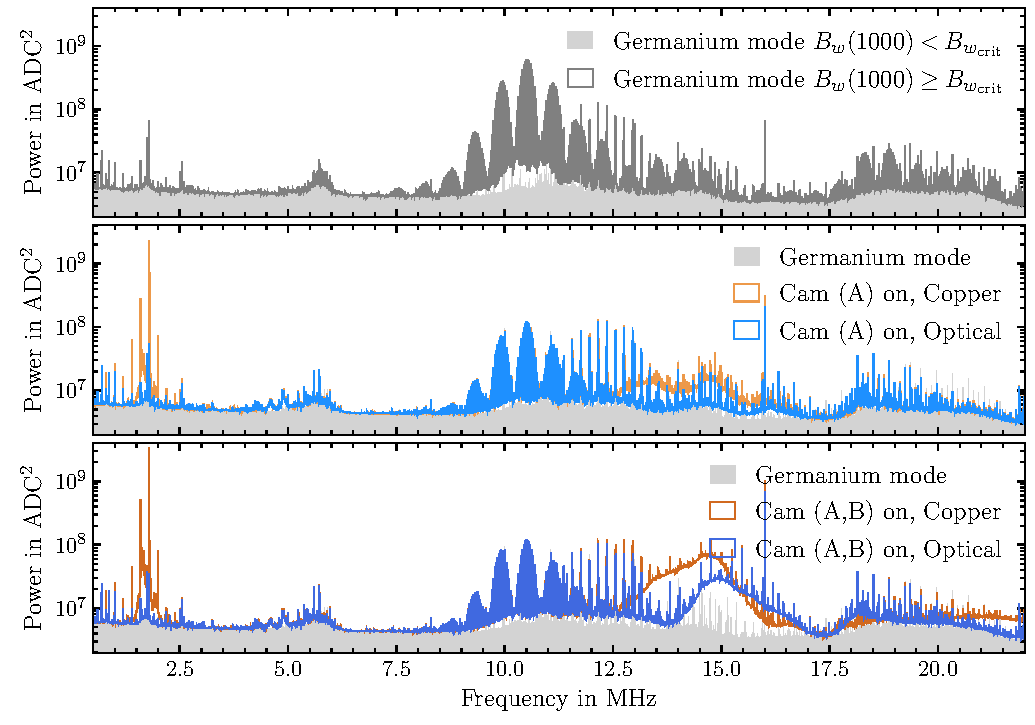
\includegraphics[width=6in]{figs/integration/ffts_5_modes.pdf}
    \caption{FFTs of the five hardware configurations described in the text in the 1-20 MHz
	range. From top to bottom: burst-free and burst-dominated Germanium mode data is compared. The combination of these populations (simply Germanium mode in the second and third panel) is compared with Compton data taken with only camera (A) on and then with camera (A) and (B) on. For Compton mode data, the copper and optical results are shown. Five minutes of data is used to construct each FFT.}
    \label{fig:fft_ge}
\end{figure}

Optical isolation of the sync lines was achieved with a minimal impact to coincidence rates while reducing the abundance of bursts within a 1000-sample-window by at least a factor of 2. Therefore, the integrated ICPC - Compton Scanner system adopted this technique to synchronize the camera and germanium data streams. Nevertheless, there is no free lunch. In principle, timing information from the cameras can be used to determine the onset of the rise, $t_0$, in germanium events. While the 1\,$\upmu$s risetime of sync pulses is negligible in a 50\,$\upmu$s coincidence window, it is not within the 4\,$\upmu$s risetime window of an ICPC event. Thus, a degradation of the $t_0$ resolution, as determined from trigger times in the camera system, is expected. The main culprit of noise bursts can now be identified as camera (B). Even with the optical sync lines, the burst abundance in 1000-sample window of 15\% was considered too high and camera (B) was powered off for most of the data taking campaign. 

\section{Monitoring} \label{sec:monitoring}
\begin{figure}[H]
    \centering
    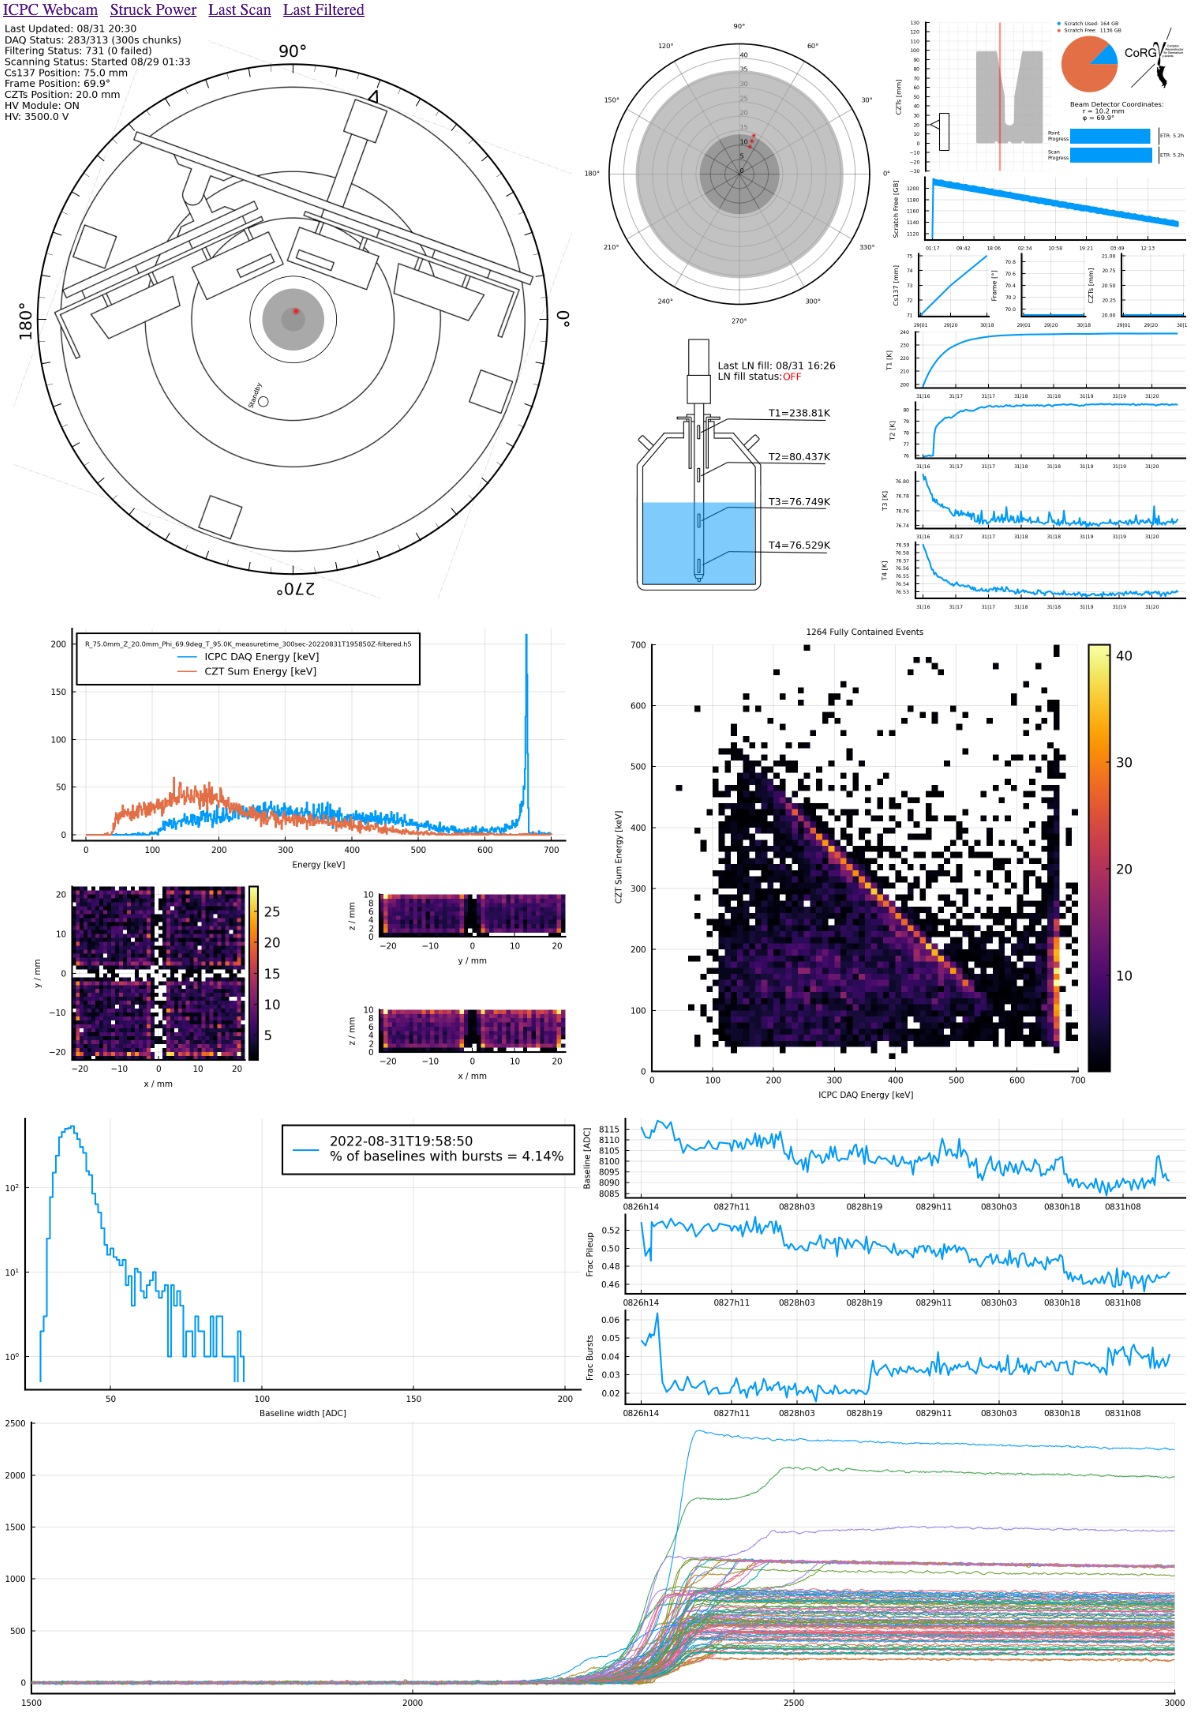
\includegraphics[width=5.4in]{figs/integration/icpc_monitor.png}
    \caption{Online monitor depicting the real-time data described in the text.}
    \label{fig:remote_monitoring}
\end{figure}

The Compton scanner and ICPC data were monitored via a web interface. The web interface consisted of multiple images which depicted real time operational and data quality parameters including motor position, LN$_2$ levels, HV status, hard drive usage, waveform baselines, burst abundance, and offline coincidence filtering status. A capture of the web interface is shown in Fig.~\ref{fig:remote_monitoring}.